% !TeX root = ..\protokoll.tex
\documentclass[../protokoll.tex]{subfiles}
\graphicspath{{\subfix{../images/}}}
\begin{document}
\part{Theorie}
\section{Weitere Vereinbarungen}
Aus dem Brechungsgesetz ergibt sich für den Winkel $\alpha$\footnote{$\alpha$ ist der Winkel zwischen dem Lot auf dem Medium 2 und dem einfallenden Strahl (vgl. \cref{fig:Brechungsgesetz}}
folgende Reihenentwicklung für $\sin \alpha$
\begin{equation}
    \sin \alpha \approx \alpha - \dfrac{\alpha^3}{3!} + \dfrac{\alpha^5}{5!} - ...
\end{equation}

In der geometrischen Optik spielen hierbei die Theorien der ersten und dritten Ordnung eine Rolle.
In der Theorie der ersten Ordnung gilt für kleine Winkel $\alpha$
\begin{equation}\label{eq:theorie-ordnung-1}
    \sin \alpha \approx \alpha
\end{equation}
Die Theorie dritter Ordnung betrachtet hierbei auch etwas größere Winkel, sodass gilt
\begin{equation}\label{eq:theorie-ordnung-3}
    \sin \alpha \approx \alpha - \dfrac{\alpha^3}{3!}
\end{equation}

\begin{figure}[H]
    \centering
    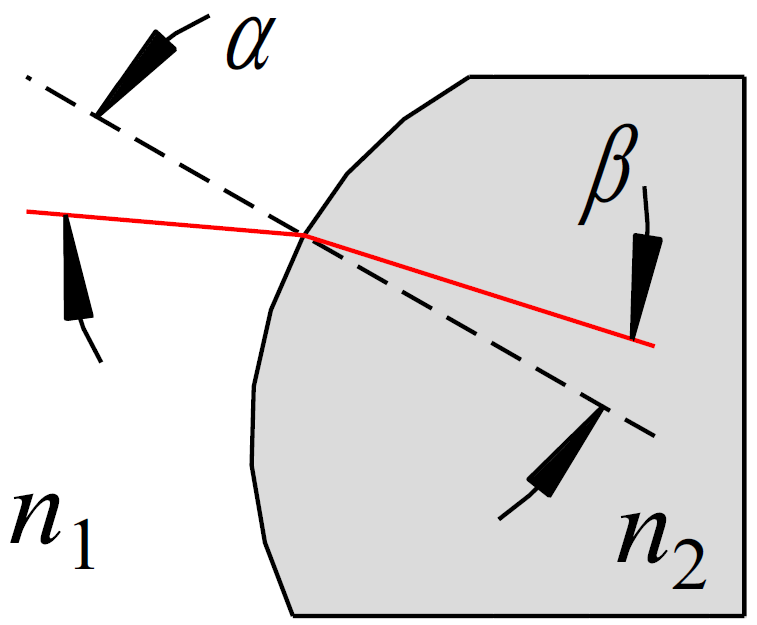
\includegraphics[width=0.2\linewidth]{2023-05-08 - V4 - Geometrische Optik, optische Abbildung und Aberrationen/images/theory/brechungsgesetz.png}
    \caption{Definition von Winkeln beim Brechungsgesetz --- \textsc{Quelle}: \cite[S. 43, Abb. 1]{script}}
    \label{fig:Brechungsgesetz}
\end{figure}
\section{Abbildungseigenschaften von Linsen}
Die Brennweite $f$ einer sphärischen Linse lässt sich mit den in der Einleitung
getroffenen Vereinbarungen mithilfe der sogenannten \textsl{Linsenmacher-Gleichung}
berechnen:
\begin{equation}\label{eq:Linsenmacher-Gleichung}
    \dfrac{1}{f} = (n - 1) \left( \dfrac{1}{R_1} - \dfrac{1}{R_2}\right)
\end{equation}
Hierbei sind gem. \cref{fig:Theorie/Linsenmacher}
\begin{itemize}[noitemsep,leftmargin=4em]
    \item[$n$:] Brechzahl des Linsenglases (abhängig von der Wellenlänge $\lambda$ des Lichts)
    \item[$R_1$:] Krümmungsradius der linken Linsenoberfläche
    \item[$R_2$:] Krümmungsradius der rechten Linsenoberfläche
\end{itemize}

Des Weiteren gilt:
\begin{itemize}[noitemsep,leftmargin=4em]
    \item[$R > 0$] wenn die Oberfläche nach links gewölbt ist\footnote{Der auf der optischen Achse liegende Punkt der Linsenoberfläche befindet sich weiter links als die übrigen Oberflächenpunkte} 
    \item[$R < 0$] wenn die Oberfläche nach rechts gewölbt ist\footnote{Der auf der optischen Achse liegende Punkt der Linsenoberfläche befindet sich weiter rechts als die übrigen Oberflächenpunkte} 
\end{itemize}

\begin{figure}[H]
    \centering
    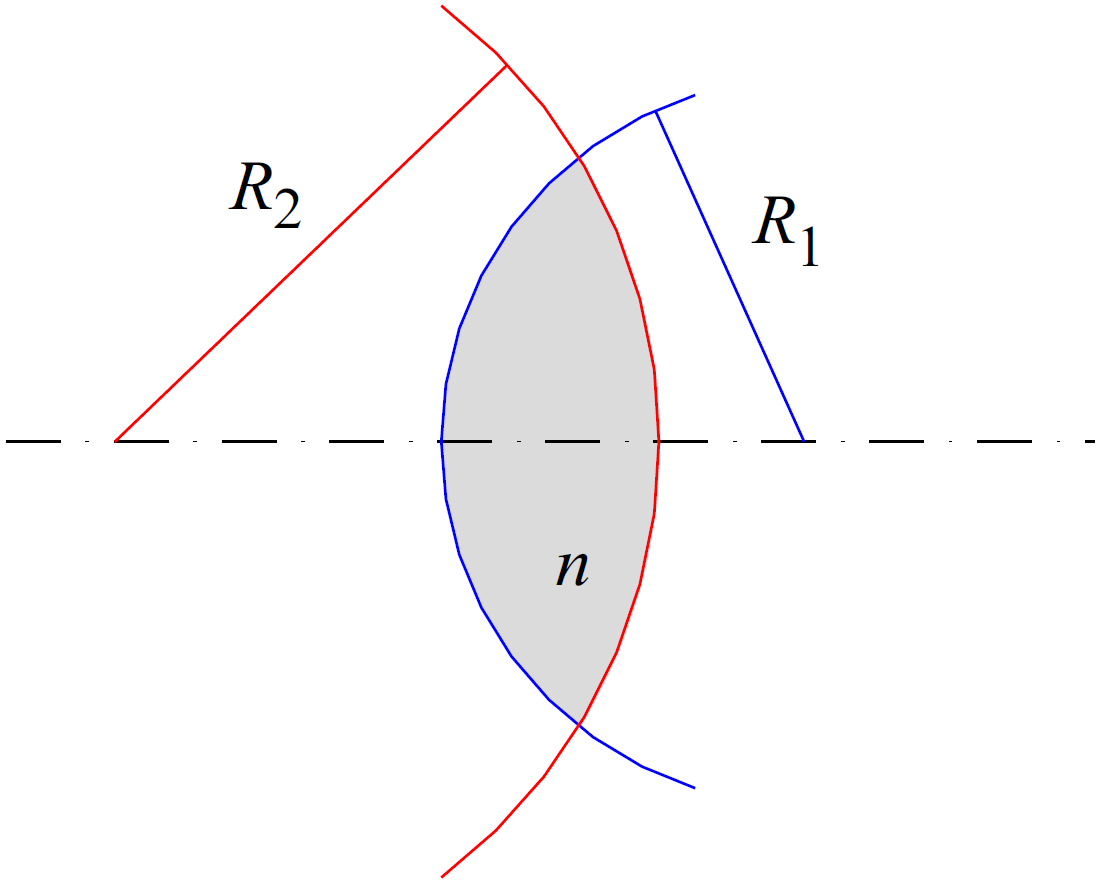
\includegraphics[width=0.25\linewidth]{2023-05-08 - V4 - Geometrische Optik, optische Abbildung und Aberrationen/images/theory/linsenmacher.png}
    \caption{Zur Definition der Vorzeichen der Krümmungsradien einer sphärischen Linse aus Glas (grau) mit der Brechzahl $n$. Im dargestellten Beispiel ist $R_1 > 0$ und $R_2 < 0$. ---
    \textsc{Quelle}: \cite[S. 44 -- Abb. 2]{script}}
    \label{fig:Theorie/Linsenmacher}
\end{figure}

Wird nun \cref{fig:Theorie/Linsengleichung} betrachtet so gilt die \textsc{Gauß}\textsl{sche Linsengleichung}:
\begin{equation}\label{eq:Gaußsche Linsengleichung}
    \dfrac{1}{f} = \dfrac{1}{g} + \dfrac{1}{b}
\end{equation}

Dabei ist:
\begin{itemize}[noitemsep,leftmargin=4em]
    \item[$g$:] Gegenstandsweite
    \begin{itemize}[noitemsep,leftmargin=4em]
        \item[$g > 0$:] reeller Gegenstand links von der Linse
        \item[$g < 0$:] virtueller Gegenstand rechts von der Linse
    \end{itemize}
    \item[$b$:] Bildweite
    \begin{itemize}[noitemsep,leftmargin=4em]
        \item[$b > 0$:] reelles Bild rechts von der Linse
        \item[$b < 0$:] virtuelles Bild links von der Linse
    \end{itemize}
\end{itemize}
Die \textsl{transversale Vergrößerung} $M$ ist gegeben durch:
\begin{equation}\label{eq:transversale Vergrößerung}
    M = \dfrac{h_b}{h_g} = - \dfrac{b}{g} = 1 - \dfrac{b}{f}
\end{equation}
mit
\begin{itemize}[nosep, noitemsep]
    \item[$h_b$:] Bildhöhe von optischer Achse aus gemessen
    \item[$h_g$:] Gegenstandshöhe von optischer Achse aus gemessen
    
    \begin{itemize}[nosep, noitemsep,leftmargin=2.25em]
        \item[$h_{b,g} > 0$,] wenn das Bild, bzw. der Gegenstand, oberhalb der optischen Achse liegen. Sonst $h_{b,g} < 0$
    \end{itemize}
\end{itemize}

Werden nun zwei \textsl{dünne Linsen} mit den Brennweiten $f_1$ und $f_2$ dicht aneinander, so gilt für die Brennweite $f$
\begin{equation}
    \dfrac{1}{f} = \dfrac{1}{f_1}+\dfrac{1}{f_2}
\end{equation}

\begin{figure}[H]
    \centering
    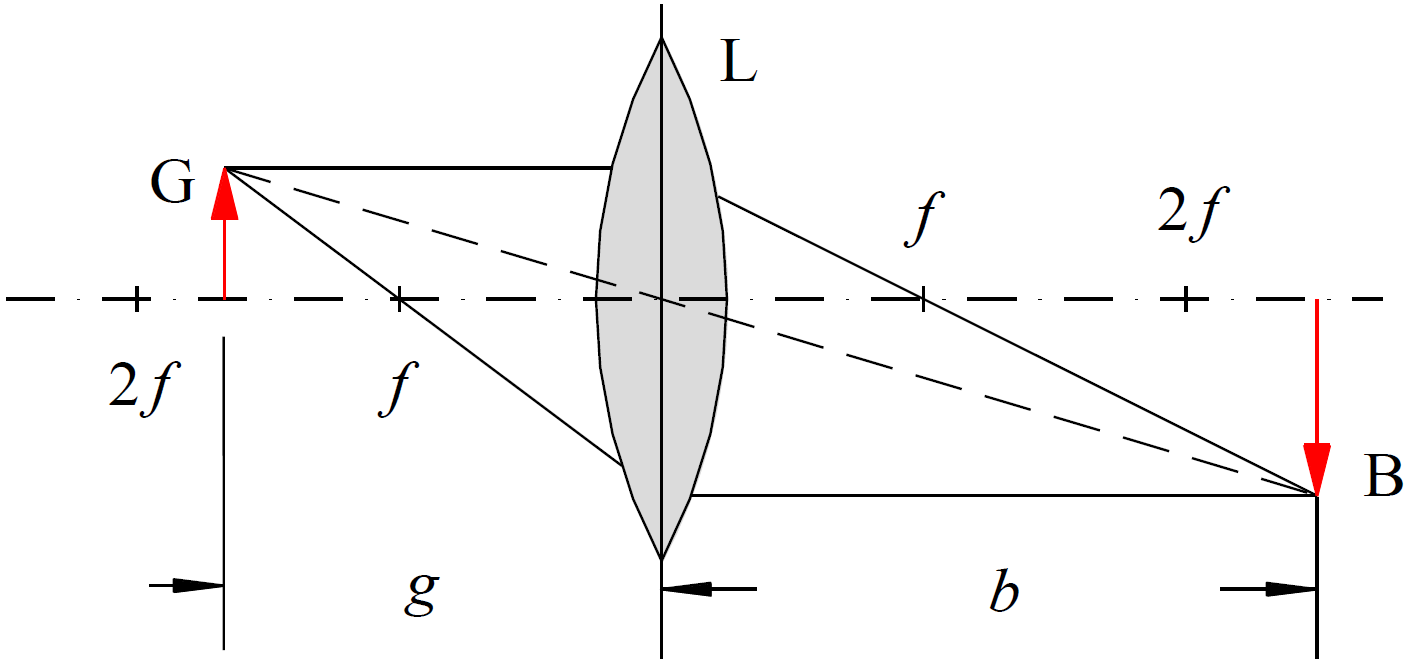
\includegraphics[width=0.4\linewidth]{2023-05-08 - V4 - Geometrische Optik, optische Abbildung und Aberrationen/images/theory/linsengleichung.png}
    \caption{Abbildung mit einer Linse L und Definition von Bezeichnungen. Bei dieser und den folgenden Abbildungen ist die Brennweite $f$ als Maß auf der optischen Achse eingetragen, deren Ursprung in der Linsenmitte liegt. ---
    \textsc{Quelle}: \cite[S. 44 -- Abb. 3]{script}}
    \label{fig:Theorie/Linsengleichung}
\end{figure}

\section{Brennweitenbestimmung mit der \textsc{Bessel}-Methode}
Mit Hilfe der \textsc{Gauß}schen Linsengleichung (vgl. Gleichung \eqref{eq:Gaußsche Linsengleichung})
kann theoretische die Brennweite einer Linse experimentell
ermittelt werden, indem für eine scharfe Abbildung die Gegenstands- und Bildweite
gemessen wird. Da jedoch die Messung dieser Größen bei kleinen Brennweiten
mit großen Unsicherheiten stattfinden kann, da die Linsenmitte als Bezugsgröße
für $b$ und $g$ schwer auszumachen ist. Daher wird in der Praxis die sogenannte
\textsc{Bessel}-Methode benutzt (vgl. \cref{fig:Bessel-Methode-Aufbau}).

\begin{figure}[H]
    \centering
    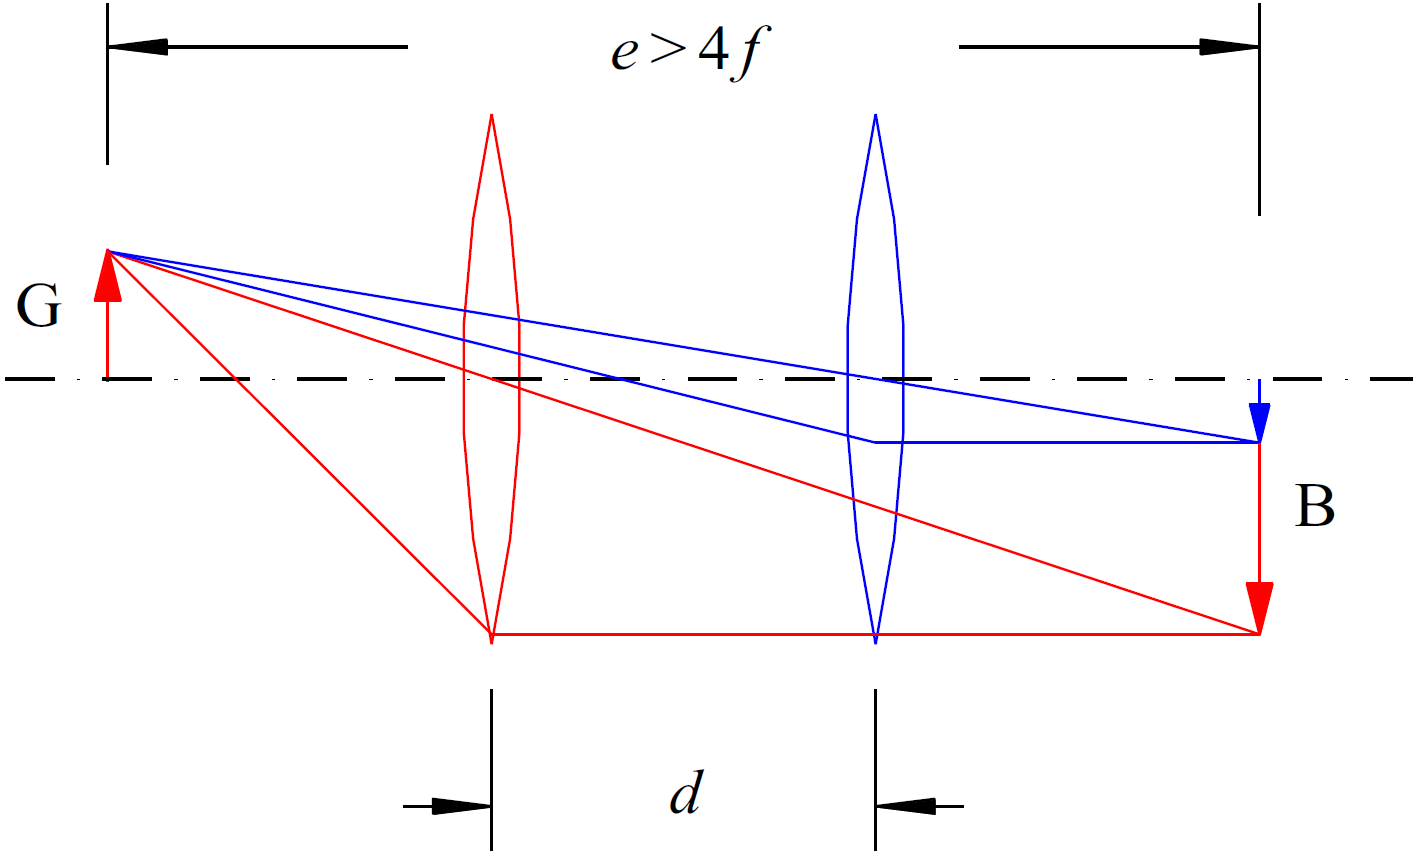
\includegraphics[width=0.3\linewidth]{2023-05-08 - V4 - Geometrische Optik, optische Abbildung und Aberrationen/images/theory/bessel-aufbau.png}
    \caption{Anordnung von Gegenstand G und Bild B bei der \textsc{Bessel}-Methode. Beim Abstand $e > 4f$ zwischen G und B gibt es zwei Linsenpositionen (rot und blau) im Abstand d, bei denen eine scharfe Abbildung erreicht wird --- \textsc{Quelle:} \cite[S. 45 -- Abb. 4]{script}}
    \label{fig:Bessel-Methode-Aufbau}
\end{figure}

Bei diesem Verfahren wird die Tatsache, dass bei der konstanten Entfernung $e > 4f$
zwischen Bild und Gegenstand zwei Linsenpositionen gibt, die zu einer scharfen Abbildung führen.
Bei einer Position findet eine Vergrößerung (rot in \cref{fig:Bessel-Methode-Aufbau}) statt, bei
der anderen eine Verkleinerung (blau in \cref{fig:Bessel-Methode-Aufbau}). Für beide
Positionen gilt:
\begin{equation}\label{eq:bessel-1}
    g + b = e
\end{equation}

Setzt man nun $b$ nach \eqref{eq:bessel-1} in \cref{eq:Gaußsche Linsengleichung} ein, so folgt:
\begin{equation}\label{eq:bessel-2}
    \dfrac{1}{g} + \dfrac{1}{e-g} = \dfrac{1}{f}
\end{equation}
woraus für $g$ folgt:
\begin{equation}\label{eq:bessel-3}
    g^2 - eg + ef = 0
\end{equation}
Diese Gleichung liefert nun zwei Lösungen für $g$, die den beiden Linsenpositionen entsprechen:
\begin{equation}\label{eq:bessel-4}
    g_{1,2} = \dfrac{e}{2} \pm \sqrt{\dfrac{e^2}{4} - ef}
\end{equation}
wobei der Abstand $d$ der beiden Positionen wie folgt berechnet werden kann
\begin{equation}\label{eq:bessel-5}
    d = g_1 - g_2 = = 2 \sqrt{\dfrac{e^2}{4} - ef}
\end{equation}
welcher auch über eine Differenzmessung einfach ermittelt werden kann.

Daraus folgt für die gesuchte Brennweite $f$
\begin{equation}
    f = \dfrac{1}{4} \left( e - \dfrac{d^2}{e} \right)
\end{equation}

\section{Abbildungsfehler}
Im Folgenden werden \textsl{sphärische} und \textsl{chromatische} Aberrationen
als zwei wichtige Abbildungsfehler vorgestellt, da diese auch in den Versuchen
vorkommen.

\subsection{Sphärische Aberration}
Sphärische Aberration tritt auf, sobald bei optischen Abbildungen der paraxaiale
Bereich verlassen wird und somit die Theorie erster Ordnung nicht mehr gilt.

Die Wirkung dieses Abbildungsfehlers lässt sich anhand \cref{fig:sphärische abberation}
für eine plankonvexe Linse verdeutlichen. Hierbei treffen parallele Strahlen die von einem
unendlich weiten Gegenstandspunkt stammen, je nach ihrem Abstand zur optischen
Achse, in diversen Winkeln auf die brechende Linsenoberfläche. Dies hat bei
einfachen sphärischen Flächen zur Folge, dass die gebrochenen Strahlen die optische
Achse in mehreren Brennpunkten trifft. Je größer der Abstand des ankommenden Strahls
zu der optischen Achse ist, desto kleiner ist die Brennweite. Eine Rechnung ergibt, dass
die Brennweite $f$ näherungsweise mit $h^2$ abnimmt, wobei $h$ der Abstand von der
optischen Achse ist. Trägt man nun $f$ über $h^2$ auf, so ergibt sich als Näherung
die folgende Geradenfunktion
\begin{equation}
    f(h) \approx f_0 - kh^2
\end{equation}
mit der Brennweite im paraxialen Bereich als $f_0$ und $k > 0$ als Konstante.

Für eine Linse mit unterschiedlichen Krümmungsradien $R_1$ und $R_2$ lässt sich die sphärische Abberation minimieren.
Hierzu wird die Linse so in den Strahlengang eingebracht, dass die Brechung auf beiden Grenzflächen möglichst gleichmäßig verteilt ist.
Für die Abbildung von unendlich weit entfernten Gegenständen müsste in \cref{fig:sphärische abberation} der linke Aufbau gewählt werden.

\begin{figure}[H]
    \centering
    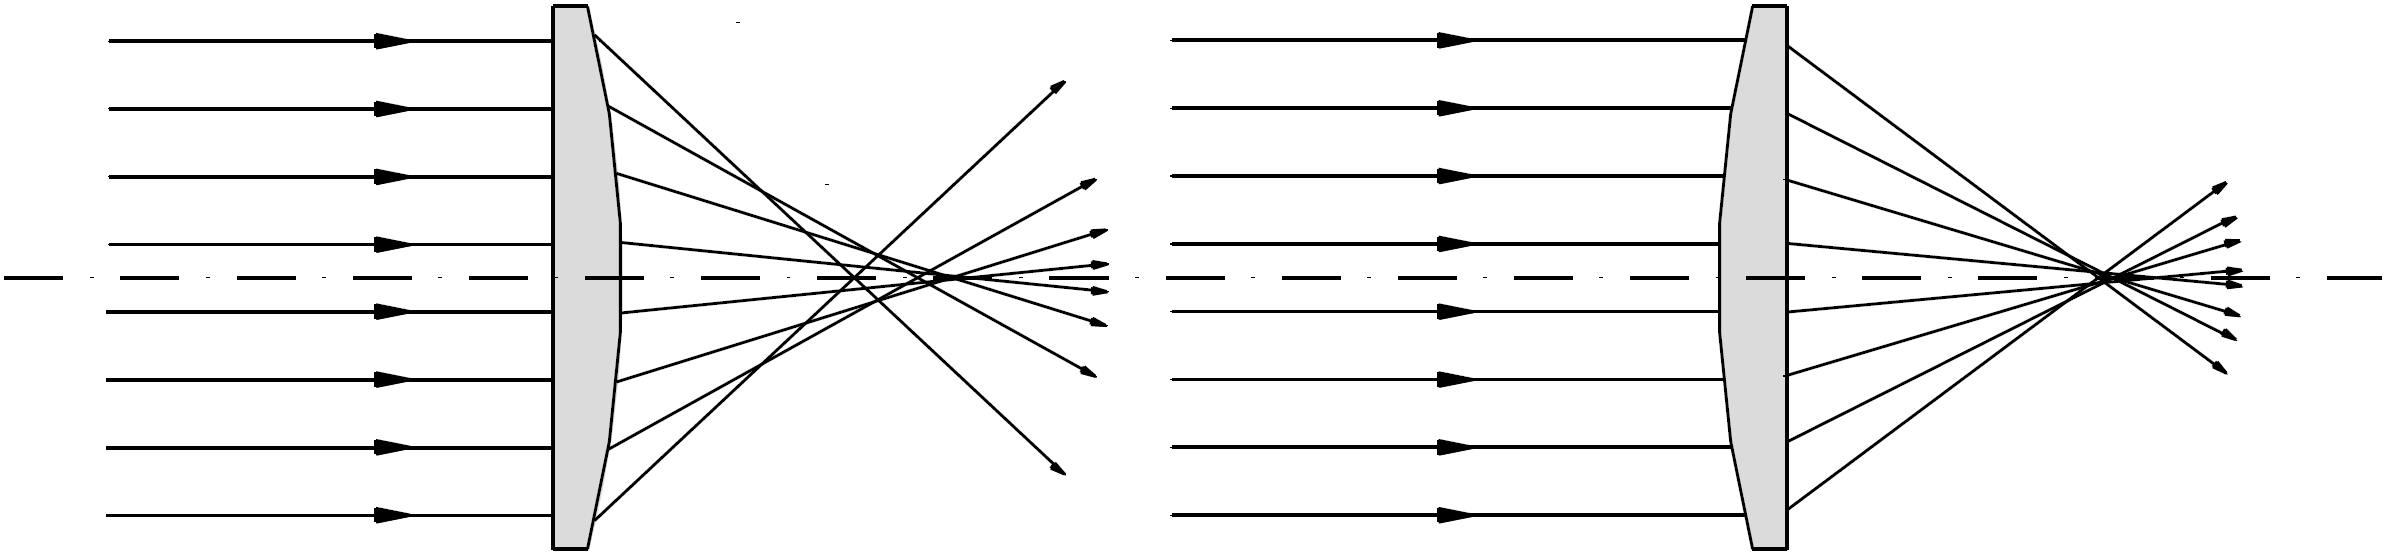
\includegraphics[width=0.4\linewidth]{2023-05-08 - V4 - Geometrische Optik, optische Abbildung und Aberrationen/images/theory/sphaerische-abberation.png}
    \caption{Auswirkunbgen der sphärischen Abberation bei verschiedenen Linsenorientierungen --- \textsc{Quelle}: \cite[S. 46, Abb. 5]{script}}
    \label{fig:sphärische abberation}
\end{figure}

Des Weiteren lässt sich die sphärische Abberation dadurch vermindern, dass vor der Linse eine Blende angebracht wird, sodass nur paraxiale
Strahlenbündel durchgelassen werden. Durch dieses Abblenden wird jedoch auch das Bild dunkler.

\subsection{Chromatische Aberration}
Chromatische Aberrationen werden durch die Abhängigkeit der Brechzahl $n$ von der Lichtwellenlänge $\lambda$
verursacht, da mit $n = n(\lambda)$ aus Gleichung \eqref{eq:theorie-ordnung-3} für $f = f(\lambda)$ folgt:
\begin{equation}
    f(\lambda) = \dfrac{1}{n(\lambda) - 1} \cdot \dfrac{R_1 R_2}{R_2 - R_1}
\end{equation}

Da die Brechzahl in Abhängigkeit der Wellenlänge mit zunehmender Wellenlänge abnimmt, nimmt $f(\lambda)$ mit $\lambda$ zu.
Das bedeutet, dass beispielsweise rotes Licht eine größere Brennweite besitzt als blaues Licht.

Die \textsc{Sellmeier}-Gleichung stellt hierbei eine gute Näherung für $n(\lambda)$ dar:
\begin{equation}
    n^2(\lambda) = 1 + B_1 \dfrac{\lambda^2}{\lambda^2 - C_1} + B_2 \dfrac{\lambda^2}{\lambda^2 - C_2} + B_3 \dfrac{\lambda^2}{\lambda^2 - C_3}
\end{equation}
wobei die Koeffizienten $B_{1,2,3}$ und $C_{1,2,3}$ experimentell bestimmt werden. Wird $\lambda$ in \unit{\mu\meter} angegeben, so lauten
die Koeffizienten für das im Praktikum verwendete N-BK7-Glas:
\begin{table}[H]
    \centering
    \begin{tabular}{l l l}
        $B_1$ = 1,03961212 & $B_2$ = 0,231792344 & $B_3$ = 1,01046945 \\
        $C_1$ = 0,00600069867 \unit{\mu\meter\squared} & $C_2$ = 0,0200179144  \unit{\mu\meter\squared} & $C_3$ = 103,560653 \unit{\mu\meter\squared}
    \end{tabular}
\end{table}

Da eine Polynom-Darstellung von $n(\lambda)$ einfacher zu handhaben ist, kann auch die folgende Näherung benutzt werden
\begin{equation}
    n(\lambda) = A_1 + A_2 \lambda + A_3 \lambda^2 + A_4 \lambda^3 + A_5 \lambda^4
\end{equation}

Wird nun $\lambda$ in \unit{\nano\meter} angegeben, so lauten die Koeffizienten $A_{1,2,3,4,5}$ für das benutzte Glas:
\begin{table}[H]
    \centering
    \begin{tabular}{l l l}
        $A_1$ = 1,74033982 & $A_2 = 1,1718506 \cdot 10^{-3} \ \unit{\per\nano\meter}$ & $A_3 = 2,3962174 \cdot 10^{-6} \ \unit{\per\nano\meter\squared}$ \\
        $A_4 = -2,263311 \cdot 10^{-9} \ \unit{\nano\meter}^{-3}$ & $A_5 = 8,1271722 \cdot 10^{-13} \ \unit{\nano\meter}^{-4}$ & 
    \end{tabular}
\end{table}

Auch chromatische Aberrationen können durch die Kombination mehrere Linsen minimiert werden, jedoch werden
im Praktikum auch nur Einzellinsen eingesetzt, wodurch es immer zu chromatischen Aberrationen kommt.

\section{Schärfentiefe}
Eine Aperturblende kann nicht nur zur Lichtbündelbegrenzung genutzt werden, sondern sie bestimmt auch die
Schärfentiefe einer Abbildung. Die dafür maßgebende Größe ist der Aperturblendendurchmesser $D$. In vielen
Fällen wird der Durchmesser nicht direkt angegeben, sondern als Blendenzahl $F$, die das Verhältnis von
Brennweite und Aperturblendendurchmesser darstellt.
\begin{equation}\label{eq:blendenzahl}
    F = \dfrac{f}{D}
\end{equation}
Ein Objektiv mit einer Brennweite von 50 mm hat beispielsweise bei einem Aperturblendendurchmesser von 25 mm
die Blendenzahl $F = 2$.

Um die Schärfentiefe zu berechnen, betrachten wir \cref{fig:schärfentiefe}.
Eine Punktlichtquelle Q mit einer Linse der Brennweite f beleuchtet den Sensor einer CCD-Kamera. von
wobei die Aperturblende mit dem Durchmesser D durch die Objektivgrenze gegeben ist. Räumlich
Die Auflösung des CCD-Sensors wird üblicherweise in Metern Schwarz/Weiß-Linienpaaren angegeben.
Vorausgesetzt, der Sensor erfasst immer noch die gleiche Breite pro Millimeter (typische Werte:

m = (100-200)/mm). Daher definieren wir die Abbildung als scharf, solange es eine solche im Bild von Q gibt.
Durchmesser d < 1/min ist.

\begin{figure}[H]
    \centering
    \includegraphics[width=0.3\linewidth]{2023-05-08 - V4 - Geometrische Optik, optische Abbildung und Aberrationen/images/theory/schärfentiefe.png}
    \caption{Zur Schärfentiefe bei der optischen Abbildung. Ist der Sensor (lila) der CCD-Kamera um die Bildweite $b$ von der
Mitte der Linse L entfernt, ergibt sich ein scharfes Bild (Bildpunkt B) der punktförmigen Lichtquelle Q. Rückt die
Kamera um $\delta b$ näher an die Linse heran (hier stark übertrieben gezeichnet), ergibt sich ein verschmiertes Bild von Q
mit dem Durchmesser $d$. --- \textsc{Quelle}: \cite[S. 49, Abb. 8]{script}}
    \label{fig:schärfentiefe}
\end{figure}
\end{document}